%%
%% FloatLab (c) 2019-23 Christopher A. Bohn
%%
%% Licensed under the Apache License, Version 2.0 (the "License");
%% you may not use this file except in compliance with the License.
%% You may obtain a copy of the License at
%%     http://www.apache.org/licenses/LICENSE-2.0
%% Unless required by applicable law or agreed to in writing, software
%% distributed under the License is distributed on an "AS IS" BASIS,
%% WITHOUT WARRANTIES OR CONDITIONS OF ANY KIND, either express or implied.
%% See the License for the specific language governing permissions and
%% limitations under the License.
%%

%%
%% (c) 2021 Christopher A. Bohn
%%

\documentclass[12pt]{article}

\usepackage{fullpage}
\usepackage{fancyhdr}
\usepackage[procnames]{listings}
\usepackage{hyperref}
\usepackage{textcomp}
\usepackage{bold-extra}
\usepackage[dvipsnames]{xcolor}
\usepackage{etoolbox}


% Customize the semester (or quarter) and the course number

\newcommand{\courseterm}{Spring 2022}
\newcommand{\coursenumber}{CSCE 231}

% Customize how a typical lab will be managed;
% you can always use \renewcommand for one-offs

\newcommand{\runtimeenvironment}{your account on the \textit{csce.unl.edu} Linux server}
\newcommand{\filesource}{Canvas or {\footnotesize$\sim$}cse231 on \textit{csce.unl.edu}}
\newcommand{\filesubmission}{Canvas}

% These are placeholder commands and will be renewed in each lab

\newcommand{\labnumber}{}
\newcommand{\labname}{Lab \labnumber\ Assignment}
\newcommand{\shortlabname}{}
\newcommand{\duedate}{}

% Individual or team effort

\newcommand{\individualeffort}{This is an individual-effort project. You may discuss concepts and syntax with other students, but you may discuss solutions only with the professor and the TAs. Sharing code with or copying code from another student or the internet is prohibited.}
\newcommand{\teameffort}{This is a team-effort project. You may discuss concepts and syntax with other students, but you may discuss solutions only with your assigned partner(s), the professor, and the TAs. Sharing code with or copying code from a student who is not on your team, or from the internet, is prohibited.}
\newcommand{\freecollaboration}{In addition to the professor and the TAs, you may freely seek help on this assignment from other students.}
\newcommand{\collaborationrules}{}

% Do you care about software engineering?

\providebool{allowspaghetticode}

\setbool{allowspaghetticode}{false}

\newcommand{\softwareengineeringfrontmatter}{
    \ifboolexpe{not bool{allowspaghetticode}}{
        \section*{No Spaghetti Code Allowed}
        In the interest of keeping your code readable, you may \textit{not} use
        any \lstinline{goto} statements, nor may you use any \lstinline{break}
        statements to exit from a loop, nor may you have any functions
        \lstinline{return} from within a loop.
    }{}
}

\newcommand{\spaghetticodepenalties}[1]{
    \ifboolexpe{not bool{allowspaghetticode}}{
        \penaltyitem{1}{for each \lstinline{goto} statement, \lstinline{break}
            statement used to exit from a loop, or \lstinline{return} statement
            that occurs within a loop.}
    }{}
}

% You shouldn't need to customize these,
% but you can if you like

\lstset{language=C, tabsize=4, upquote=true, basicstyle=\ttfamily}
\newcommand{\function}[1]{\textbf{\lstinline{#1}}}
\setlength{\headsep}{0.7cm}
\hypersetup{colorlinks=true}

\newcommand{\startdocument}{
    \pagestyle{fancy}
    \fancyhf{}
    \lhead{\coursenumber}
    \chead{\ Lab \labnumber: \labname}
    \rhead{\courseterm}
    \cfoot{\shortlabname-\thepage}

	\begin{document}
	\title{\ Lab \labnumber}
	\author{\labname}
	\date{Due: \duedate}
	\maketitle

    \textit{\collaborationrules}
}

\newcommand{\rubricitem}[2]{\item[\underline{\hspace{1cm}} +#1] #2}
\newcommand{\bonusitem}[2]{\item[\underline{\hspace{1cm}} Bonus +#1] #2}
\newcommand{\penaltyitem}[2]{\item[\underline{\hspace{1cm}} -#1] #2}

%%
%% labs/common/semester.tex
%% (c) 2021-22 Christopher A. Bohn
%%
%% Licensed under the Apache License, Version 2.0 (the "License");
%% you may not use this file except in compliance with the License.
%% You may obtain a copy of the License at
%%     http://www.apache.org/licenses/LICENSE-2.0
%% Unless required by applicable law or agreed to in writing, software
%% distributed under the License is distributed on an "AS IS" BASIS,
%% WITHOUT WARRANTIES OR CONDITIONS OF ANY KIND, either express or implied.
%% See the License for the specific language governing permissions and
%% limitations under the License.
%%


% Customize the semester (or quarter) and the course number

\newcommand{\courseterm}{Fall 2022}
\newcommand{\coursenumber}{CSCE 231}

% Customize how a typical lab will be managed;
% you can always use \renewcommand for one-offs

\newcommand{\runtimeenvironment}{your account on the \textit{csce.unl.edu} Linux server}
\newcommand{\filesource}{Canvas or {\footnotesize$\sim$}cse231 on \textit{csce.unl.edu}}
\newcommand{\filesubmission}{Canvas}

% Customize for the I/O lab hardware

\newcommand{\developmentboard}{Arduino Nano}
%\newcommand{\serialprotocol}{SPI}
\newcommand{\serialprotocol}{I2C}
%\newcommand{\displaymodule}{MAX7219digits}
%\newcommand{\displaymodule}{MAX7219matrix}
\newcommand{\displaymodule}{LCD1602}

\setbool{usedisplayfont}{true}

\newcommand{\obtaininghardware}{
    The EE Shop has prepared ``class kits'' for CSCE 231; your class kit costs \$30.
    The EE Shop is located at 122 Scott Engineering Center and is open M-F 7am-4pm. You do not need an appointment.
    You may pay at the window with cash, with a personal check, or with your NCard.
    The EE shop does \textit{not} accept credit cards.
}

% Update to reflect the CS2 course(s) at your institute

\newcommand{\cstwo}{CSCE~156, RAIK~184H, or SOFT~161}

% Do you care about software engineering?

\setbool{allowspaghetticode}{false}

% Which assignments are you using this semester, and when are they due?

\newcommand{\pokerlabnumber}{1}
\newcommand{\pokerlabcollaboration}{
    Sections~\ref{sec:connecting}, \ref{sec:terminology}, \ref{sec:gettingstarted}, \ref{subsec:typesofpokerhands}, and~\ref{subsec:studythecode}: \freecollaboration
    Sections~\ref{sec:completingcard} and~\ref{subsec:completepoker}: \individualeffort
}
\newcommand{\pokerlabdue}{Week of August 29, before the start of your lab section}

\newcommand{\keyboardlabnumber}{2}
\newcommand{\keyboardlabcollaboration}{\individualeffort}
\newcommand{\keyboardlabdue}{Week of January 31, before the start of your lab section}

\newcommand{\pointerlabnumber}{3}
\newcommand{\pointerlabcollaboration}{\individualeffort}
\newcommand{\pointerlabdue}{Week of February 7, before the start of your lab section}

\newcommand{\integerlabnumber}{4}
\newcommand{\integerlabcollaboration}{\individualeffort}
\newcommand{\integerlabdue}{Week of February 14, before the start of your lab section}

\newcommand{\floatlabnumber}{5}
\newcommand{\floatlabcollaboration}{\individualeffort}
\newcommand{\floatlabdue}{soon}

\newcommand{\addressinglabnumber}{6}
\newcommand{\addressinglabcollaboration}{\individualeffort}
\newcommand{\addressinglabdue}{Week of February 28, before the start of your lab section}

%bomblab was 7
%attacklab was 8

\newcommand{\pollinglabnumber}{9}
\newcommand{\pollinglabcollaboration}{\individualeffort}
\newcommand{\pollinglabdue}{Week of April 11, before the start of your lab section}
\newcommand{\pollinglabenvironment}{your \developmentboard-based class hardware kit}

\newcommand{\ioprelabnumber}{\pollinglabnumber-prelab}
\newcommand{\ioprelabcollaboration}{\freecollaboration}
\newcommand{\ioprelabdue}{Before the start of your lab section on April 5 or 6}

\newcommand{\interruptlabnumber}{10}
\newcommand{\interruptlabcollaboration}{\individualeffort}
\newcommand{\interruptlabdue}{Week of April 18, before the start of your lab section}
\newcommand{\interruptlabenvironment}{your \developmentboard-based class hardware kit}

\newcommand{\capstonelab}{ComboLock}    % this will come into play when we generalize capstonelab
\newcommand{\capstonelabnumber}{11}
\newcommand{\capstonelabcollaboration}{\teameffort}
\newcommand{\capstonelabdue}{Week of May 2, Before the start of your lab section\footnote{See Piazza for the due dates of teams with students from different lab sections.}}
\newcommand{\capstonelabenvironment}{your \developmentboard-based class hardware kit}

\newcommand{\memorylabnumber}{12}
\newcommand{\memorylabcollaboration}{This is an individual-effort project. You may discuss the nature of memory technologies and of memory hierarchies with classmates, but you must draw your own conclusions.}
\newcommand{\memorylabdue}{Week of May 2, at the end of your lab section}
\newcommand{\memorylabenvironment}{your \developmentboard-based class hardware kit and your account on the \textit{csce.unl.edu} Linux server}

% Labs not used this semester

\newcommand{\concurrencylabnumber}{XX}
\newcommand{\concurrencylabcollaboration}{\individualeffort}
\newcommand{\concurrencylabdue}{not this semester}

\newcommand{\ssbcwarmupnumber}{XX}
\newcommand{\ssbcwarmupcollaboration}{\freecollaboration}
\newcommand{\ssbcwarmupdue}{not this semester}

\newcommand{\ssbcpollingnumber}{XX}
\newcommand{\ssbcpollingcollaboration}{\individualeffort}
\newcommand{\ssbcpollingdue}{not this semester}

\newcommand{\ssbcinterruptnumber}{XX}
\newcommand{\ssbcinterruptcollaboration}{\individualeffort}
\newcommand{\ssbcinterruptdue}{not this semester}

%%
%% labs/common/storylines.tex
%% (c) 2020-23 Christopher A. Bohn
%%
%% Licensed under the Apache License, Version 2.0 (the "License");
%% you may not use this file except in compliance with the License.
%% You may obtain a copy of the License at
%%     http://www.apache.org/licenses/LICENSE-2.0
%% Unless required by applicable law or agreed to in writing, software
%% distributed under the License is distributed on an "AS IS" BASIS,
%% WITHOUT WARRANTIES OR CONDITIONS OF ANY KIND, either express or implied.
%% See the License for the specific language governing permissions and
%% limitations under the License.
%%

\newcommand{\MeetArchie}{
    \begin{wrapfigure}{r}{0.33\textwidth}
        \centering
        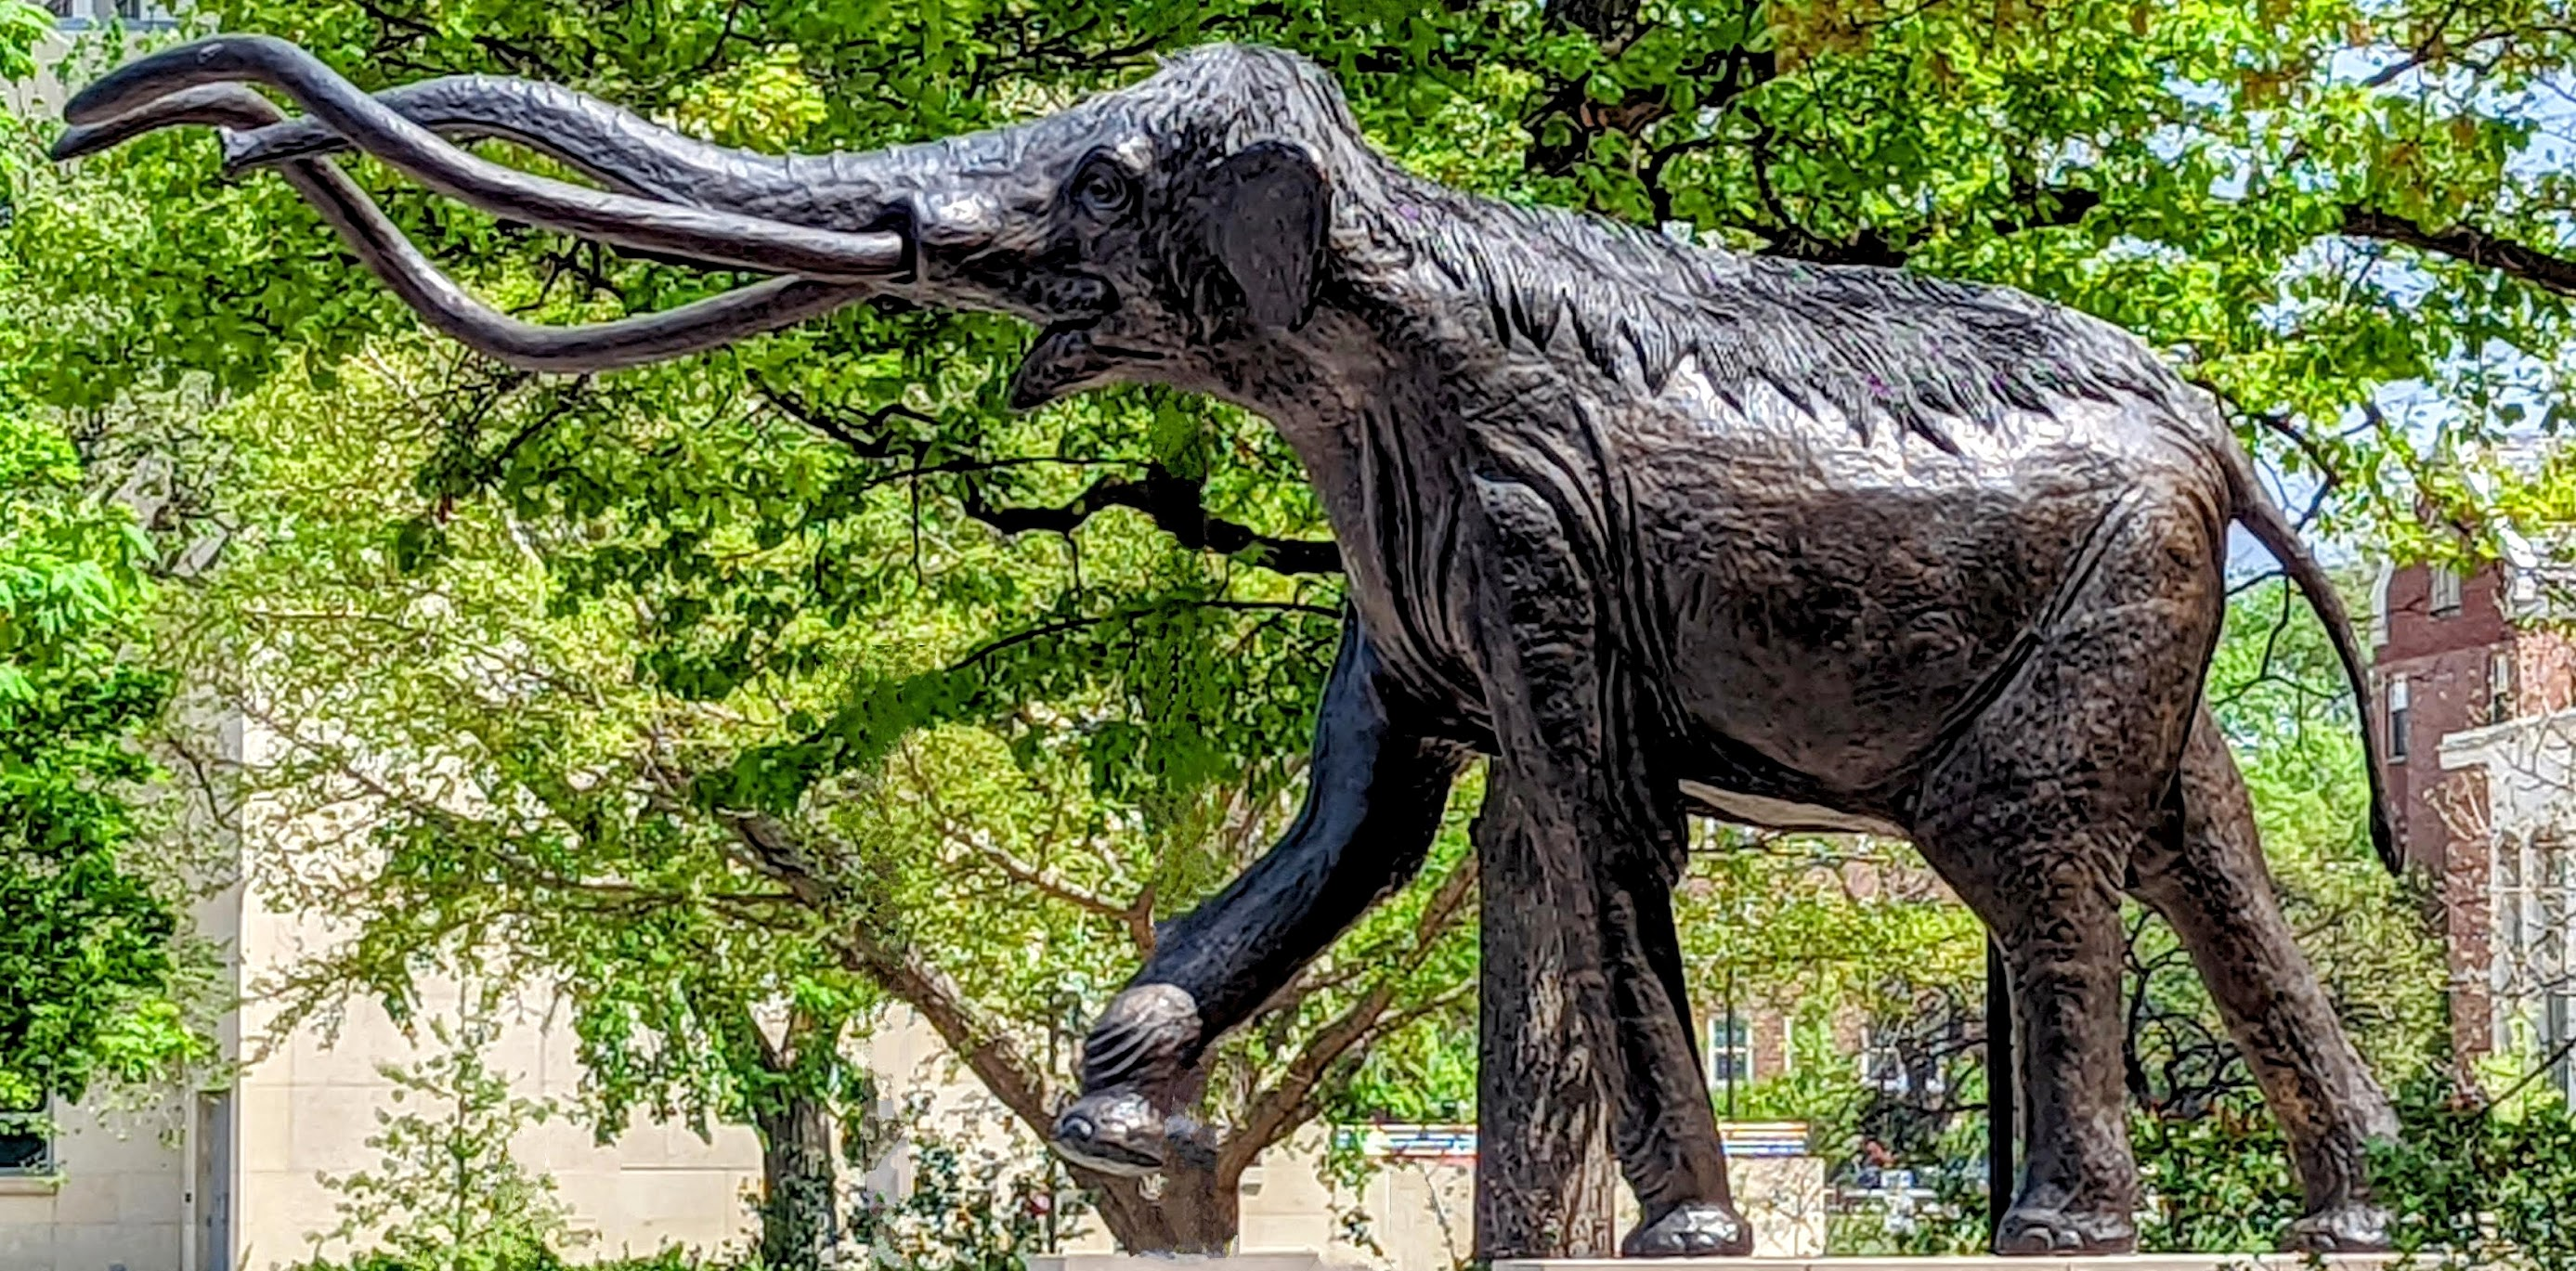
\includegraphics[width=.4\textwidth]{archie}
        \caption{Archie.\\ \footnotesize{Photograph by Bohn.}}
    \end{wrapfigure}

    You're relaxing at your favorite hangout when another customer catches your attention.
    He's rather large (dare I say, \textit{mammoth}), a bit hairy, and looking frustrated in front of his laptop.
    ``I'm Archie,'' he says, ``and I'm trying to teach myself this card game called \textit{Poker}.
    I found this source code that I thought I could use to understand Poker better, but the code is incomplete, and I don't entirely understand what's there.
    Could you explain the code to me, please?'
}

\newcommand{\GetHired}{
    Archie's face lights up in a very big smile.
    ``Thanks!''
    After pausing in thought for a moment, he says, ``Say, I've got a new startup company that could really use your help.
    Are you interested?
    It'll be exciting!''
}

\newcommand{\FirstDayOnTheJob}{
    \begin{wrapfigure}{r}{0.33\textwidth}
        \centering
        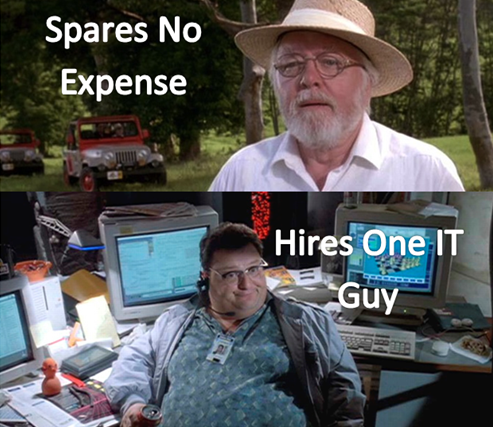
\includegraphics[width=.4\textwidth]{some-expenses-spared}
        \caption{Some expenses were spared.\\ \footnotesize{Original images \textcopyright\ Universal Studios and Amblin Entertainment, Inc. Meme creator unknown.}}
    \end{wrapfigure}

    You've recently been hired to help get the Pleistocene Petting Zoo get started.
    Your new employer, Archie, is surprisingly honest: he admits to you that some expenses were spared.
    Archie cheerfully points out that any challenge is also an opportunity to succeed.
    You suspect your job will offer plenty of ``opportunities to succeed.''
}

\newcommand{\HasKeyboard}{
    Great news!
    Archie brings you your new keyboard.
    He also brings you a problem of his own.
    Because you were held up with the broken keyboard, Archie decided to try some programming on his own, and his code is behaving strangely.
}

\newcommand{\ArchieWroteSmellyCode}{
    Working at the Pleistocene Petting Zoo certainly is proving to be interesting.
    You're glad that you don't have to worry about the problem of the giant sloths very slowly chasing their handlers, but now it seems that Archie has decided to try to write a program or two.
    At a glance, his code is smellier than the wooly rhinoceros' enclosure.
    But you take a closer look anyway to try to understand why his code acts strangely.
}

\newcommand{\InsurancePreview}{
    You hear somebody enter the room.
    ``\textit{Frankenstein}, `boat','' is the challenge, and she answers, ``borne.''
    Archie introduces you to the new arrival, ``Lil, this is our new developer, the one who wrote the app we just used.''
    He turns to you: ``This is Lilith Redd from business operations.''
    He turns back to her and continues, ``Lil, what's the good word?''

    ``The word isn't good, I'm afraid.
    I just heard back from the insurance company.''
}

\newcommand{\OnLoanToEclecticElectronics}{
    All work at the Pleistocene Petting Zoo has stopped while Archie tries to find a $\cancelto{\mathrm{reasonable}}{\mathrm{gullible}}$ insurance company.
    Rather than furloughing staff, he's asked everybody to help out with his other startup companies for a week or two.
    He specifically asked that you help out with Eclectic Electronics.

    Herb Bee, the chief engineer, explains that Eclectic Electronics is developing a patent-pending C-licon tool that will convert C code into an integrated circuit that has the same functionality as the original C code.
    To test it out, he tasked you with writing the code to implement an Arithmetic Logic Unit (ALU).
    Your task will be to implement integer addition, subtraction, multiplication, and division.
    Even though high-level languages' \textit{logical} boolean operations normally are not part of an ALU, Herb wants you to include these in the ALU to see if that can make some programs run faster.
    Because bitwise operations and bit shift operations have been implemented, you will be able to use C's bitwise and bit shift operators, but because arithmetic operations have not yet been implemented, you cannot use C's arithmetic operators.
    Because C library functions generally make use of arithmetic operations (which have not yet been implemented), you cannot use library functions.
}

\newcommand{\SuccessfulALU}{
    Herb smiles as he hands you the the test results from the latest integrated circuit fab batch.
    ``C-licon successfully turned your code into an ALU.
    Nicely done!''
    I think maybe it's time to use C-licon to see if we can improve the Floating Point Unit (FPU) on our experimental microprocessor.
}

\newcommand{\WriteAnFPU}{
    Herb tells you that, Eclectic Electronics tested the integrated circuit that the C-licon tool created from your ALU code, and they've concluded that C-licon is ready to use for their new experimental microprocessor.
    He tasks you with writing C code (that will be used by the C-licon tool) to implement a Floating Point Unit (FPU).
    Your task will be to implement floating point addition, subtraction, multiplication, and division.
    You can use any bit operations and, thanks to the ALU you wrote, you can use any integer arithmetic operations (use the conventional + - * / operators).
    Because the FPU has not yet been implemented, you cannot use C's floating point operations, you cannot use \lstinline{float}s nor \lstinline{double}s, and you cannot use library functions.
}

\newcommand{\GoingBackToTheZoo}{
    Lil enters the room.
    Herb challenges her: ``\textit{Gulliver's Travels}, `endian','' and Lil answers, ``ends.''

    Lil walks up to you and says, ``We have the insurance situation taken care of, and it's time to get the Zoo ready for guests.
    We're reassembling the tech team, and there's plenty of work to do.''

    You smile.
    ``That's good news!''

    Lil's face is hard to read.
    ``Well, yes and no.
    It's good that you'll be able to resume work on the Zoo's systems.
    But while Archie was waiting for us to fix the insurance situation, he got bored and -- cutting a long story short -- he ended up creating some new `opportunities' that we need you `to succeed' at.''
}

\newcommand{\SettledIntoRoutine}{
    You've settled into a comfortable routine at the Pleistocene Petting Zoo.
    While your job isn't quite as exciting as that of the saber-toothed tigers' dentist, it still has something new and interesting almost every day.

    Archie announces that he heard that hand-crafted assembly code can be faster than high-level language code.
    You try to explain that while this may have been true decades ago, modern optimizing compilers generate code faster than what a typical programmer can achieve with assembly code.
    Archie doesn't believe you and insists that you write the zoo's new cipher program in x86 assembly code.
}

\newcommand{\NewmanRanOffWithSamples}{
    Archie is hurriedly packing is trunk, like he's about to leave on a short-notice urgent trip.
    Before charging out the door, he pauses to tell you, ``Newman just stole some of our samples.
    I need to track him down before he sells them to the Supersized Safari Syndicate.
    I guess this means you're in charge of the Zoo's computer system now.
    Don't worry, you'll be fine. What could possibly go wrong?''
}

\newcommand{\BombLabIntroduction}{  % Ties Bryant & O'Halloran's Bomb Lab into the Pleistocene Petting Zoo story
    In a jarring collision of movie franchises, the CEO of Virtucon makes a Zoom call to the Pleistocene Petting Zoo.
    For some reason that nobody really explains, you're the only person available to handle the situation.
    The guy, who sounds kind of like an animated ogre, demands that the Pleistocene Petting Zoo deliver to him a megalodon shark with a head-mounted laser capable of emitting a beam of pure antimatter.

    You blurt out, ``Then it's not a laser,'' and then try to explain to him that megalodons are from the Miocene epoch, and expecting to find them at the Pleistocene Petting Zoo would be as ridiculous as a Cretaceous-period tyrannosaur at a Jurassic-themed park.

    ``Zip it!'' commands the guy who kind of looks like the host of a public-access show you used to watch.
    ``Since you won't meet my demand, my minions have placed a `binary bomb' under your zoo.
    Because I like really convoluted plans, we put software on your Linux server that controls the bomb.
    If you do nothing, the bomb will explode.
    If you turn off the Linux server, the bomb will explode.
    If you go slower than 50mph, the bomb will -- no, never mind that last part.

    ``The bomb software consists of a sequence of phases.
    Each phase expects you to type a particular string on \texttt{stdin}.
    If you type the correct string, then the phase is {\em defused} and the bomb proceeds to the next phase. Otherwise, the bomb {\em explodes}.
    The bomb is defused when every phase has been defused.

    ``Your mission, which you have no choice but to accept, is to defuse your bomb before the due date.
    Good luck, and welcome to the bomb squad!''
}

\newcommand{\FoodLockersAreStuck}{
    Having saved the Zoo from Dr. Evil's binary bomb, you relax back in your chair and think about taking a break.
%SPRINGBREAK
    Maybe an entire week in which you don't have solve any problems or meet any deadlines -- that'd be real nice.
%FALLBREAK
    % Maybe 4-day weekend in which you don't have solve any problems or meet any deadlines -- that'd be real nice.

    Another Zoom call comes in.
    \textit{What now!?} you wonder as you take your feet off of the desk to answer the call.
    An uncomfortable-looking animal handler says, ``We can't unlock the food lockers.
    It's the animals' feeding time, and we can't open the food lockers!
    It's feeding time, we can't get to the animals' food, and,'' his eyes dart nervously toward the animal enclosures, ``and many of them have sharp, pointy claws and others have big, stompy feet.''
}

\newcommand{\AttackLabIntroduction}{    % Ties Bryant & O'Halloran's Attack Lab into the Pleistocene Petting Zoo story
    You managed to keep the Pleistocene Petting Zoo from blowing to smithereens, but it turns out that Dr. Evil's minions weren't too careful when they put the bomb control software on the Zoo's Linux server.
    The software that controls the food locker has been heavily damaged!
    The functions that unlock the food locker doors are still present, but there's no way to activate those functions.

    You then recall what Archie told you when he hired you: some expenses were spared.
    You run the machine code through a disassembler and quickly see that it has a buffer overflow vulnerability.
    Before the situation in the dire wolf enclosure gets too dire, you sit down and get to work.

    The \function{ctarget} code runs on an older machine that allows executable code to be present on the stack, so it's vulnerable to a conventional code injection buffer overflow attack.
    \begin{itemize}
        \item Phase 1 (\function{touch1}) unlocks the food locker so the animal handlers can prepare the food.
        \item Phase 2 (\function{touch2}) opens the doors between the food locker and the carnivore enclosures;
        you will need to pass a cookie to the function to authenticate yourself.
        \item Phase 3 (\function{touch3}) closes the doors between the food locker and the carnivore enclosures.
    \end{itemize}
    The \function{rtarget} code runs on a newer machine that does not allow executable code to be present on the stack, so you'll have to conduct a return-oriented programming attack on it.
    \begin{itemize}
        \item Phase 4 (\function{touch2)} opens the doors between the food locker and the herbivore enclosures;
        you will need to pass a cookie to the function to authenticate yourself.
        \item Phase 5 (\function{touch3}) closes the doors between the food locker and the herbivore enclosures.
    \end{itemize}
}

\newcommand{\MostAnimalsAreFed}{
    Before you take on the Phase 5, pause to consider what you have accomplished so far.
    In Phases 2 and 3, you caused a program to execute machine code of your own design.
    If {\sc ctarget} had been a network server, you could have injected your own code into a distant machine.
    In Phase 4, you circumvented two of the main devices modern systems use to thwart buffer overflow attacks.
    Although you did not inject your own code, you were able inject a type of program that operates by stitching together sequences of existing code.
    Also, all animals have been fed, the carnivores are still in their enclosure, the mammoths can't fit through the herbivore door, and only the giant sloths seem interested in very slowly escaping.
}

\newcommand{\ArchieReturns}{
    Archie returns from tracking down Newman, who'd run off with some of the Pleistocene Petting Zoo's samples shortly before Dr.~Evil's Zoom call.
    ``It turns out he didn't get very far at all,'' Archie sighs.
    ``He ran into a flock of terror birds as he was leaving, and we found him in one of the emergency shelters.

    Archie smiles. ``I trust things were uneventful while I was away?''
}

\newcommand{\PickingUpNewmansProject}{
    Archie seems genuinely surprised that Newman is refusing to go back to work.
    ``You would think that he'd be grateful for being rescued from that flock of terror birds.''
    Before you can wonder out-loud whether it would be a good idea to trust someone who had just tried to sell trade secrets to a competitor, Archie gives you your new task.

    ``Because Newman isn't cooperating, I need you to finish the project he was working on.
    As you can imagine, duplicating the genetic information for our exhibits can take a long time, and Newman realized that we might be able to duplicate the data faster if we had a concurrent program which has one thread reading from the original data and another thread writing the copy.
    Unfortunately, he ran off to sell samples to the  Supersized Safari Syndicate before finishing the duplicator.
    Right now the duplicator seems to work, but it usually makes imperfect copies.
    Have you ever seen a paleolama with two noses, four eyes, and no ears!?''
}

\newcommand{\WeNeedBetterDetection}{
    Between Newman trying to sell samples to a competitor, that weird guy almost blowing up the zoo, and the animals almost escaping, Archie is getting worried.
    ``I think we need to introduce additional protective measures.
    As useful as your challenge-response app is in helping us detect intruders, I think it's now clear that we need something that will detect someone -- or some\textit{thing} -- when they're someplace they shouldn't be, even when no one else is around.
    I've asked the team at Eclectic Electronics to put something together.''
}

\newcommand{\WeNeedBetterLocks}{
    Between Newman trying to sell samples to a competitor, that weird guy almost blowing up the zoo, and the animals almost escaping, Archie is getting worried.
    ``I think we need to introduce additional protective measures.
    As useful as your challenge-response app is in helping us detect intruders, I think it's now clear that we need something that will keep someone -- or some\textit{thing} -- out of places they shouldn't be, even when no one else is around.
    I've asked the team at Eclectic Electronics to put something together.''
}

\newcommand{\IntroduceHardware}{
    Archie walks up to you, along with Herb Bee from Eclectic Electronics.
    Herb is holding a tangled mess of electronics.
    Archie explains, ``Herb here has developed a prototype of a device that he thinks will be useful for our physical security needs, as well as a few other applications around here. He calls it the \textit{Cow Pi}.''

% TODO: parameterize based on which microcontroller is actually being used
    You look at the device in Herb's hands and see the \nano\ central to the circuit.
    ``Isn't \textit{-Pi} typically used as a suffix for circuits that use a Raspberry Pi instead of an Arduino?''

    Herb replies, ``Typically, yes, but \textit{Cowduino} isn't very punny, is it?''

    Archie chimes in, ``Maybe with the right emphasis: \textit{Cow-DOO-ino}.''

    ``That's kind of subtle, don't you think? How will people know to put the emPHAsis on that sylLAble?''

    ``I think we're getting off topic here,'' you point out.
    ``How can I help?''

    ``Oh, right,'' Herb says, ``We'd like you to kick its proverbial tires.
    Let's start off with something simple, like a number builder tool.''
}

\newcommand{\JeffGoldblum}{
    Herb looks over your work.
    ``Hmm, yes. I think this is coming along nicely.
    Let's run a few more tests.''

    Archie storms into the room.
    ``We have \textit{got} to do something about security!
    How's that doodad coming along?
    Because there's now a half-man/half-fly in the labs going on-and-on about Chaos Theory and how if we just give him a MacBook and a spaceship then he'll be able to get the Lord of Thunder to travel across the 8th Dimension.
    Is that thing just about ready?''

    Herb shakes his head, ``No, not quite yet. It should be ready in about a week.''
}

\newcommand{\DisdainfulHerb}{
    Smoke wafts from Herb's soldering iron as he looks up when you approach.
    Cleaning the iron's tip, he quotes:
    ``Somebody once said, `The three most dangerous things in the world are a programmer with a soldering iron, a hardware engineer with a software patch, and'{}'' -- he glances nervously in Archie's direction -- ``{}`a user with an idea.'\footnote{
        Rick Cook, \textit{The Wizardry Consulted}, 1995.
    }$^{\mathrm{,}}$\footnote{
        The notion of being wary of programmers wielding screwdrivers or soldering irons long pre-dated this quote, as there are apocryphal tales of people who found it easier to modify the hardware to suit the software rather than the other way around.
    }''
}

\newcommand{\NumberConversionTool}{     % Since we're now allowing `sprintf()` with the LCD1602, converting between decimal and hexadecimal is trivial; it still might be okay for 7-segment displays
    Herb gets straight to the point.
    ``We promised Archie that we'd be able to start using the Cow Pi to build systems in a week.
    So far we've tested its input/output functionality, but we still need to test its timer and also whether we can take inputs without constantly polling the input devices.
    As before, we don't need to do anything too fancy;
    let's try a number base conversion tool.''
}

\newcommand{\LessDisdainfulHerb}{
    Smoke wafts from Herb's soldering iron as he looks up when you approach.
    Cleaning the iron's tip, he notes:
    ``Somebody once said that one of the most dangerous things in the world is a programmer with a soldering iron.''\footnote{
        ``The three most dangerous things in the world are a programmer with a soldering iron, a hardware engineer with a software patch, and a user with an idea.'' -- Rick Cook, \textit{The Wizardry Consulted}, 1995.
    }$^{\mathrm{,}}$\footnote{
        The notion of being wary of programmers wielding screwdrivers or soldering irons long pre-dated this quote, as there are apocryphal tales of people who found it easier to modify the hardware to suit the software rather than the other way around.
    }
}

\newcommand{\RemoteControlledCar}{

    About this time, Archie walks by, thinking about electric carts to transport visitors around the Pleistocene Petting Zoo.
    ``They probably should be remote-controlled.''
    He looks at you and Herb, and asks, ``Do you think you could make a cart a remote-controlled cart?''

    You ask the obvious question, ``Are there carts here already?''

    Archie waves his hand in the air, dismissing that detail, ``Not yet, but could you make the remote-control?''
    
    You hestatingly summarize: ``You want a cartless remote-controlled cart?''

    Archie beamingly smiles, ``Exactly!''

    Herb jumps in, ``Yes, we'll do it.''
    Herb looks at you and adds, ``It'll give us a chance to test the Cow Pi's timer and whether we can take inputs without constantly polling the input devices.''
}

\newcommand{\LauraDern}{
    You and Herb look for Archie in the Pleistocene Petting Zoo's labs to give him the good news, and you find a blond woman wearing cargo shorts, butchering a Gilbert and Sullivan song\dots \\ \\
    \textmusicalnote\ I am the very model of a modern vice admiral \textmusicalnote \\
    \textmusicalnote\ I've information about all things paleobotanical \textmusicalnote \\
    \textmusicalnote\ And I've been up to my armpits in problems scatological \textmusicalnote \\
    \textmusicalnote\ During the regency I had experience matriarchical \textmusicalnote \\
    \textmusicalnote\ I plot space travel, normal and superluminal \textmusicalnote \\
    \textmusicalnote\ (Even if I challenge the Pauli exclusion principle) \textmusicalnote \\

    ``I don't know how these people keep getting into our labs.
    \textit{Please} tell me that you have good news,'' pleads Archie.

    ``Yes, the Cow Pi is ready for whatever you need: calculators, security systems, parking meters -- you name it,'' Herb cheerfully responds.

    ``Excellent.''
    Archie turns to you.
    ``I'd like you and Newm... no, \textit{not} Newman.
    I'd like you and someone else on the staff to get started right away.
    Here's what I'd like to have built first.''
}

\newcommand{\CalculatorNeeded}{
    ``I have various teams working on different projects around here to improve security,'' Archie reminds you.
    He glances toward the Zoo's labs, where there's now a guy who looks like the actor who portrayed the fictional actor who portrayed the Norse god Odin, trying to avoid children while wistfully talking about raising rabbits in Montana.
    You briefly wonder why there are children someplace where there are also carnivorous megafauna, and then you remember that you work at a petting zoo.
    ``What I need your team to do,'' Archie continues, ``is make a four-function calculator so that we can quickly and easily determine whether we have the correct number of specimens, or if any are missing.''
}

\newcommand{\CalculatorCounting}{
    Technicians are using your calculator to compute how many specimens are still present in the lab, and establish that all specimens are accounted for after Newman's attempted theft.
    As reports come in of facilities getting secured with Cow Pi-based locks and passages being monitored with Cow Pi-based motion sensors, Archie smiles and tells you that this was a job well done.
    With all of the excitement neatly wrapped-up and arriving at a satisfactory conclusion, you look forward to a boring career in which there's absolutely no screaming and running for your life.
}

\newcommand{\CombinationLockNeeded}{
    ``I have various teams working on different projects around here to improve security,'' Archie reminds you.
    He glances toward the Zoo's labs, where there's now a guy who looks like the actor who portrayed the fictional actor who portrayed the Norse god Odin, trying to avoid children while wistfully talking about raising rabbits in Montana.
    You briefly wonder why there are children someplace where there are also carnivorous megafauna, and then you remember that you work at a petting zoo.
    ``What I need your team to do,'' Archie continues, ``is make a combination lock so that only authorized people can get into our lab facilities.''
}

\newcommand{\CombinationLockInstalled}{
    After fastening the new electronic combination lock to the lab door, Archie smiles and tells you that this was a job well done.
    With all of the excitement neatly wrapped-up and arriving at a satisfactory conclusion, you look forward to a boring career in which there's absolutely no screaming and running for your life.
}

\newcommand{\RangeFinderNeeded}{
    ``I have various teams working on different projects around here to improve security,'' Archie reminds you.
    He glances toward the Zoo's labs, where there's now a guy who looks like the actor who portrayed the fictional actor who portrayed the Norse god Odin, trying to avoid children while wistfully talking about raising rabbits in Montana.
    You briefly wonder why there are children someplace where there are also carnivorous megafauna, and then you remember that you work at a petting zoo.
    ``What I need your team to do,'' Archie continues, ``is make a range finder that will alert us when someone -- or some\textit{thing} -- gets too close to someplace they shouldn't be.''
}

\newcommand{\RangeFinderDetecting} {
    A technician installing a new range finder outside the lab door briefly sets off the alarm, but then the range finder falls quiet and faithfully reports that nothing is approaching.
    As reports come in of facilities getting secured with Cow Pi-based locks, and of accurate speciment counts accomplished with Cow Pi-based calculators, Archie smiles and tells you that this was a job well done.
    With all of the excitement neatly wrapped-up and arriving at a satisfactory conclusion, you look forward to a boring career in which there's absolutely no screaming and running for your life.
}


\renewcommand{\labnumber}{\floatlabnumber}
\renewcommand{\labname}{Floating Point Representation and Arithmetic Lab}
\renewcommand{\shortlabname}{floatlab}
\renewcommand{\collaborationrules}{\floatlabcollaboration}
\renewcommand{\duedate}{\floatlabdue}

\pagelayout
\begin{document}
    \labidentifier\

    \pdfbookmark[1]{Frontmatter}{frontmatter}                           In this assignment, you will write code for \runtimeenvironment\ that will use new electronic devices to interact with the physical world.

The instructions are written assuming you will edit the code in the Arduino IDE and run it on \runtimeenvironment, constructed according to the pre-lab instructions.
If you wish, you may edit the code in a different environment; however, our ability to provide support for problems with other IDEs is limited.

\section*{Learning Objectives}

After successful completion of this assignment, students will be able to:
\begin{itemize}
    \item Work collaboratively on a hardware/software project
    \item Design and implement a simple embedded system
    \item Expand their programming knowledge by consulting documentation
\end{itemize}

\subsection*{Continuing Forward}

This penultimate lab assignment does not contribute to the final lab assignment.
By integrating elements of what you learned in this course, and by demonstrating that you can review documentation to learn on your own, to design a small embedded system, you will show how much progress you have made this semester.

\section*{During Lab Time}

During your lab period, coordinate with your group partner(s) to decide on your working arrangements.
Unless you're only going to work on the assignment when you're together, you may want to set up a private Git repository that is shared with your partner(s).
With your partner(s), modify your hardware kit as described in Section~\ref{sec:hardwareMods}.
Then, think through your system's design and begin implementing it.
The TAs will be available for questions.


    \softwareengineeringfrontmatter

    \section*{Scenario}                                                 \WriteAnFPU

    \section{Assignment Summary}                                        This assignment is principally about getting comfortable when explicitly working with memory.
Being able to think about a value and a reference to that value distinctly will improve your programming skills in any language.

Before you do so, in Section~\ref{sec:archiesCode} you will examine Archie's code.
Parts of Archie's programs use code that the C standard explicitly states will result in undefined behavior.
By understanding the mistakes that Archie made, we hope that you can avoid them in your own code.

In Section~\ref{sec:challengeResponse}, you will build and use a linked list.
This will require you to allocate space for the list's nodes and manipulate pointers that connect the nodes to each other.

\ifboolexpe{not bool{allowspaghetticode}}{
    There are no particular restrictions in this assignment other than those common to most lab assignments in this course.
    You can check whether you're using a \lstinline{goto} or \lstinline{continue} statement, or whether you're using \lstinline{break} or \lstinline{return} to exit a loop, by running the constraint-checking Python script:
    \texttt{python constraint-check.py linkedlistlab.json}
}{}


    \section{Getting Started}                                           Download \textit{\shortlabname.zip} or \textit{\shortlabname.tar} from \filesource\ and copy it to \runtimeenvironment.
Once copied, unpackage the file.
Four of the five files (\textit{alu.h}, \textit{basetwo.c}, \textit{alu.c}, and \textit{integerlab.c}) contain the starter code for this assignment.
The last file (\textit{Makefile}) tells the \texttt{make} utility how to compile the code.
To compile the program, type:

\texttt{make}

This will produce an executable file called \textit{integerlab}.

When you run the program with the command \texttt{\textbf{\textit{./integerlab}}}, you will be prompted:

\begin{verbatim}
    Enter a one- or two-operand logical expression,
        a two-operand comparison expression, a two-operand arithmetic expression,
        "lg <value>" or "exponentiate <value>" to test your powers-of-two code,
        "is_negative <value>" to determine if 2's complement value is negative,
        "add1 <binary_value1> <binary_value2> <carry_in>" for 1-bit full adder,
        "add32 <hex_value1> <hex_value2> <carry_in>" for 32-bit ripple-carry adder,
        or "quit":
\end{verbatim}

When you enter a value, if it is prepended with \texttt{\textbf{\textit{0x}}} then the parser will parse it as a hexadecimal value;
otherwise, except as noted in Sections~\ref{subsec:one-bit-full-adder} and \ref{subsec:ripple-carry-adder}, the parser will treat it as a decimal value.

For now, type \texttt{\textbf{\textit{quit}}} to exit the program.

\subsection{Description of IntegerLab Files}

\subsubsection{integerlab.c}

Do not edit \textit{integerlab.c}.

This file contains the driver code for the lab.
It parses your input, calls the appropriate arithmetic function, and displays the output.

\subsubsection{alu.h} \label{subsubsec:alu.h}

Do not edit \textit{alu.h}.

This header file contains two type definitions:
\begin{description}
    \item[one\_bit\_adder\_t] is a structure to hold the 1-bin inputs (\lstinline{a}, \lstinline{b}, \lstinline{c_in}) and 1-bit outputs (\lstinline{sum}, \lstinline{c_out}) of a one-bit full adder.
    \item[alu\_result\_t] is a structure to hold the outputs from an arithmetic logic unit.
        Its fields are:
        \begin{itemize}
            \item \lstinline{result}, a 16-bit bit vector that is considered ``the'' result of the computation
            \item \lstinline{supplemental_result}, a 16-bit bit vector that stores additional result data from instructions that place their results in two registers
            \item \lstinline{unsigned_overflow}, a 1-bit flag to indicate whether overflow occurred when interpreting the source operands as unsigned values
            \item \lstinline{signed_overflow}, a 1-bit flag to indicate whether overflow occurred when interpreting the source operands as signed values
            \item \lstinline{divide_by_zero}, a 1-bit flag to indicate whether there was an attempt to divide by zero.
        \end{itemize}
\end{description}

The header file also contains two macros, \function{is_zero()} and \function{is_not_zero()} to bootstrap your ALU code.
These macros act like functions and return a boolean value to indicate whether an integer is 0 or not.\footnote{
    The astute student will quickly realize that \function{is_not_zero()} is not necessary and, with a little thought, will realize that they can \function{is_zero()} as a function within the constraints of this assignment.}

The header file also contains several function declarations.
The requirements for these functions will be discussed later in this assignment.

\subsubsection{basetwo.c}

This is the first of two files that you will edit.

There are two functions in \textit{basetwo.c} that will allow you to demonstrate an understanding of powers-of-two and/or an understanding of some uses of bit shifts.
\begin{description}
    \item[lg()] returns the base-2 logarithm of its argument, assuming its argument is a positive power-of-two;
        if the argument is 0 or is not a power-of-two, then there are no guarantees about the function's return value
    \item[exponentiate()] creates a power-of-two by raising 2 to the provided exponent, assuming the exponent is a non-negative value strictly less than 32;
        if the argument is negative or is greater than 31, then there are no guarantees about the function's return value
\end{description}
These functions are inverses of each other: $x = \log_2 2^x$, and $y = 2^{\log_2 y}$.

Strictly speaking, you can write your ALU code without these functions;
however, some students in the past had difficulty finding solutions for their ALU code without obtaining a base-2 logarithm and/or calling a function to create a power-of-two.
Rather than tempt you to violate one of the assignment's constraints by calling the \textit{math} library's \function{log2()}, \function{exp2()}, and/or \function{pow()} functions, we now have you write your own code for these functions.

\subsubsection{alu.c}

This file will contain most of the code that you write, and the functions in \textit{alu.c} are in the order in which you will likely write them.
\begin{itemize}
    \item A simple check
        \begin{description}
            \item[is\_negative()] returns a boolean value to indicate whether the argument, when interpreted as a signed integer, is negative
        \end{description}
    \item Equality comparisons
        \begin{description}
            \item[equal()] returns \lstinline{true} if and only if $value1 = value2$
            \item[not\_equal()] returns \lstinline{true} if and only if $value1 \not = value2$
        \end{description}
    \item Logical operations
        \begin{description}
            \item[logical\_not()] returns the logical inverse of the argument
            \item[logical\_and()] returns the logical conjunction of the two arguments
            \item[logical\_or()] returns the logical disjunction of the two arguments
        \end{description}
    \item Addition and subtraction
        \begin{description}
            \item[one\_bit\_full\_addition()] performs addition for one bit position, determining both the sum bit and the carry-out bit
            \item[ripple\_carry\_addition()] adds two 32-bit values to each other and to a carry-in bit
            \item[add()] adds two 16-bit values to each other
            \item[subtract()] subtracts a 16-bit value from another
        \end{description}
    \item Inequality comparisons
        \begin{description}
            \item[less\_than()] returns \lstinline{true} if and only if $value1 < value2$
            \item[at\_most()] returns \lstinline{true} if and only if $value1 \leq value2$
            \item[at\_least()] returns \lstinline{true} if and only if $value1 \geq value2$
            \item[greater\_than()] returns \lstinline{true} if and only if $value1 > value2$
        \end{description}
    \item Unsigned multiplication and division
        \begin{description}
            \item[multiply\_by\_power\_of\_two()] multiplies the first argument by the second, assuming that the second argument is zero or a power of two;
                there are no guarantees if this assumption is not satisfied
            \item[unsigned\_multiply()] multiplies two 16-bit values to each other, if the arguments are interpreted as unsigned integers
            \item[unsigned\_divide()] divides a 16-bit value by another, if the arguments are interpreted as unsigned integers
        \end{description}
    \item Signed multiplication and division (bonus credit)
    \begin{description}
        \item[signed\_multiply()] multiplies two 16-bit values to each other, if the arguments are interpreted as signed integers
        \item[signed\_divide()] divides a 16-bit value by another, if the arguments are interpreted as signed integers
    \end{description}
\end{itemize}


    \section{Constants and Queries} \label{sec:constantsAndQueries}     \subsection{Constants}

There are seven named constants in \textit{fpu.c}.

\begin{description}
    \checkoffitem{Assign the appropriate bit vectors to \lstinline{SIGN_BIT_MASK}, \lstinline{EXPONENT_BITS_MASK}, and \lstinline{FRACTION_BITS_MASK} so that you can use them to mask-off the sign bit, the exponent bits, and the fraction bits, respectively, in a \lstinline{ieee754_t} floating point value.}
    \checkoffitem{Assign the single-precision exponent bias to \lstinline{EXPONENT_BIAS} and assign to \lstinline{NUMBER_OF_FRACTION_BITS} the number of bits used for the fraction bit field in a single-precision floating point number.}
    \checkoffitem{Assign to \lstinline{NAN} and \lstinline{INFINITY} suitable bit vectors for single-precision Infinity and Not-a-Number.}
\end{description}

These constants will not be graded directly;
they exist solely to make your code more readable.
You may define additional named constants as needed.

\subsection{Query Functions}

There are three functions to identify whether an \lstinline{ieee754_t} floating point value is neither normal nor subnormal.
The remaining query function determins whether an \lstinline{ieee754_t} floating point value is negative.
\begin{description}
    \checkoffitem{Implement \function{is_nan()} to detect whether a value is Not-a-Number without regard to the value's sign.}
    \begin{itemize}
        \item Note that \function{is_nan()} must return \lstinline{true} for \textit{all} valid NaN bit vectors and not just those that match your \lstinline{NAN} constant.
    \end{itemize}
    \checkoffitem{Implement \function{is_nan()} to detect whether a value is infinity without regard to the value's sign.}
    \checkoffitem{Implement \function{is_nan()} to detect whether a value is zero without regard to the value's sign.}
    \checkoffitem{Implement \function{is_negative()} to detect whether a value is negative.}
\end{description}


    \section{Examining IEEE 754-Compliant Values}                       \subsection{Printing a IEEE~754-Compliant Value} \label{subsec:printing}

Examine the stub for \function{ieee754_to_string()}.
This function prints its \lstinline{ieee754_t} argument bit vector in hexadecimal, and then it is supposed to print the bit vector as a binary floating point value.
Making use of the query functions that you wrote, the stub prints the sign and handles the special cases.

Find this code:

\begin{lstlisting}
// The number is either Normal or Subnormal
unsigned int integer = 0;
uint32_t fraction = 0;
int exponent = 0;
char fraction_string[40];
/* DETERMINE THE INTEGER PORTION, THE FRACTION, AND THE EXPONENT */
\end{lstlisting}

Assign the appropriate values to \lstinline{integer}, \lstinline{fraction}, and \lstinline{exponent}.
The \lstinline{integer} is the implicit integer portion of the significand.
The \lstinline{fraction} is simply the fraction bits as they appear in the \lstinline{number}.
The \lstinline{exponent} is the two's complement representation of the exponent that you get after removing the bias from the \lstinline{number}'s \texttt{E} field.
Do not make any assignments to \lstinline{fraction_string} -- this is a buffer that will be used later.
The subsequent \function{sprintf()} call uses these variables to print the bit vector as a binary floating point value.

\paragraph*{Check Your Work}

Compile and run \texttt{\textbf{\textit{./floatlab}}}, trying a few values, starting with values whose IEEE~754 representation are easy to check.
For example:

\begin{verbatim}
        Enter a value, a two-operand arithmetic expression,
            "denormalize <value> <change exponent amount>",
            "renormalize <value> <change exponent amount>",
            or "quit": 1
        0x3f800000	+1.0000,0000,0000,0000,0000,000_{2} x 2^{0}

        Enter a value, ... or "quit": .25
        0x3e800000	+1.0000,0000,0000,0000,0000,000_{2} x 2^{-2}

        Enter a value, ... or "quit": 15.625
        0x417a0000	+1.1111,0100,0000,0000,0000,000_{2} x 2^{3}
\end{verbatim}

Try a few more on your own.
You can also try creating some bit vectors to see that the sign, significand, and exponent are all what you expect, based on your understanding of the IEEE~754 format.
For example:

\begin{verbatim}
        Enter a value, ... or "quit": 0xF22AAAAA
        0xf22aaaaa	-1.0101,0101,0101,0101,0101,010_{2} x 2^{101}
\end{verbatim}

Don't forget to check subnormal numbers, too.
For example:

\begin{verbatim}
        Enter a value, ... or "quit": 5e-40
        0x000571cc	+0.0000,1010,1110,0011,1001,100_{2} x 2^{-126}
\end{verbatim}

\subsection{\texttt{unnormal\_t} and its functions} \label{subsec:unnormal}

The \lstinline{unnormal_t} data type is a structure with fields for the sign bit, the integer portion, the fractional portion, and the exponent.
It also has flags for Not-a-Number and for Infinity.
Unlike the IEEE~754 format, an \lstinline{unnormal_t} value can have more than one bit in its integer portion.

You should \textit{not} access the \lstinline{unnormal_t} fields directly.
Instead, use the \function{unnormal()} macro to create an \lstinline{unnormal_t} value, the accessor functions that we provide to retrieve the fields, and the modifier functions that we provide to make adjustments in a value-preserving manner.

\textit{\textbf{NOTE:}} while you typically will see non-primitive variables passed by reference to C functions, the \lstinline{unnormal_t} functions use pass-by-value.
This is considerably less efficient in both time and memory (and there are other downsides beyond the scope of what you've learned so far);
however, passing the \lstinline{unnormal_t} variables by value ensures that there will be no aliased variables and also that memory management will be handled by the program stack.
This means that the variables passed as arguments to functions will be unchanged, and if an \lstinline{unnormal_t} variable is returned then it will be a modified copy of the original.
A consequence of this is that \textit{you must make sure that you always use the value returned by a function if you expect to use the effect of the function.}

You can, and should, look at the functions' signatures in \textit{unnormal.h}.
We summarize the functions here:

\begin{itemize}
    \item Creating and printing an \lstinline{unnormal_t} value (all necessary calls to these functions are in the starter code)
    \begin{description}
        \item[unnormal()] returns an \lstinline{unnormal_t} value (\textit{not} a pointer) based on the arguments provided.
            The argument list is a series of dot-prefixed named fields (such as \lstinline{.sign=0, .infinity=1}) whose meanings are the obvious ones from the class discussion about floating point numbers.
            \textit{\textbf{Note: }} the \lstinline{.exponent} argument, if included, is expected to be a two's complement value.
            \textit{\textbf{Note: }} the \lstinline{.fraction} argument, if included, is expected to be the numerator of $\frac{.fraction\ argument}{2^{64}}$ (\textit{i.e.}, the $2^{-1}$ bit is $bit_{63}$)\@.
        \item[unnormal\_to\_string] returns a string representation of the value.
            Because of the number of bits available in the \lstinline{unnormal_t} fields, the significand is represented in base-16, though the exponent is the exponent of 2.
    \end{description}
    \item Accessors
    \begin{description}
        \item[get\_sign()] returns 0 if the value is positive, 1 if the value is negative
        \item[get\_integer()] returns a \lstinline{uint64_t} storing the unsigned integer representation of the value's integer portion
        \item[get\_fraction()] returns a \lstinline{uint64_t} storing the numerator of $\frac{get\_fraction()}{2^{64}}$ (\textit{i.e.}, the $2^{-1}$ bit is $bit_{63}$)
        \item[get\_exponent()] returns a \lstinline{int16_t} storing the two's complement representation of the exponent
        \item[is\_infinite()] returns 0 if the value is finite (or NaN), 1 if the value is $\pm\infty$
        \item[is\_not\_a\_number()] returns 0 if the value is a valid number, 1 if the value is not a number
    \end{description}
    \item Bit shifts (some of these functions are equivalent to each other, to support whichever mental model works for you)
    \begin{description}
        \item[shift\_left\_once()] aka \function{decrement_exponent()}, aka \function{move_binary_point_to_the_right()} -- shifts the significand's bits to the left by one position, having the effect of moving the binary point to the right and decreasing the exponent by one
        \item[shift\_right\_once()] aka \function{increment_expoennt()}, aka \function{move_binary_point_to_the_left()} -- shifts the significand's bits to the right by one position, having the effect of moving the binary point to the left and increasing the exponent by one
        \item[shift\_left()] shifts the significand's bits to the left by a specified amount
        \item[shift\_right()] shifts the significand's bits to the right by a specified amount
    \end{description}
    \item Alignment functions (shifts bits by specifying the desired result instead of the amount)
    \begin{description}
        \item[place\_all\_bits\_in\_integer()] aka \function{prepare_for_arithmetic()} shifts the significand such that the least-significant \lstinline{1} bit is in the $2^0$ position, with a corresponding change in the exponent (the fraction, of course, will be 0)
        \item[set\_integer()] if possible, shifts the significand such that the resulting integer portion is the specified value, with a corresponding changes in the fraction and exponent
        \item[set\_exponent()] shifts the significand, with a corresponding change in the exponent, such that the resulting exponent is the specified value
    \end{description}
    \item Static Warnings (warnings based on the current bit positions)
    \begin{description}
        \item[multiplication\_is\_not\_recommended()] indicates that there are \lstinline{1} bits to the right of the binary point:
                if there are \lstinline{1} bits in the fraction, then there will be extra bookkeeping that you will be responsible for;
                we recommend that you attempt multiplication only when all \lstinline{1} bits are in the integer portion
        \item[multiplication\_is\_unreliable()] indicates that there are \lstinline{1} bits far enough to the left of the binary point that multiplication could yield a product whose integer portion exceeds the available bits
        \item[addition\_is\_unreliable()] indicates that there are \lstinline{1} bits far enough to the left of the binary point that addition could yield a sum whose integer portion exceeds the available bits
    \end{description}
    \item Dynamic Warnings (warnings that result from the last function call)
    \begin{description}
        \item[shift\_overflowed()] indicates that one or more \lstinline{1} bit shifted to the left beyond the available bits
        \item[shift\_underflowed()] indicates that one or more \lstinline{1} bit shifted to the right beyond the available bits
        \item[operation\_was\_not\_performed()] indicates that the previous function did not have the desired result, such as attempting to shift by a negative amount or attempt to set an integer value whose bits are not present in the significand
        \item[created\_number\_is\_improbable()] indicates that a call to \function{unnormal()} was made with all of the fraction's \lstinline{1} far enough from the binary point that it is unlikely to have been the intended value (because it is \textit{possible} that the requested fraction is also the intended fraction, an Unnormal value with the requested fraction was created)
    \end{description}
    \item Prediction Functions (warnings that indicate what will happen in the next operation)
    \begin{description}
        \item[fraction\_will\_carry\_into\_integer\_on\_addition()] indicates that if the next operation is addition with the specified values, then adding the fractions will carry into the integer portion, requiring you to add 1 to the sum's integer
        \item[fraction\_will\_borrow\_from\_integer\_on\_subtraction()] indicates that if the next operation is subtraction with the specified values, then subtracting the fractions will require ``borrowing'' from the integer portion, requiring you to subtract 1 to the difference's integer
        \item[left\_shift\_will\_make\_multiplication\_unreliable()] indicates that if the next function is \function{left_shift_once()} (or one of its aliases) then after that function call, \function{multiplication_is_unreliable()} will return \lstinline{true}
        \item[left\_shift\_will\_make\_addition\_unreliable()] indicates that if the next function is \function{left_shift_once()} (or one of its aliases) then after that function call, \\ \function{addition_is_unreliable()} will return \lstinline{true}
        \item[left\_shift\_will\_overflow()] indicates that if the next function is \function{left_shift_once()} (or one of its aliases) then after that function call, \function{shift_overflowed()} will return \lstinline{true}
        \item[right\_shift\_will\_underflow()] indicates that if the next function is \function{right_shift_once()} (or one of its aliases) then after that function call, \function{shift_underflowed()} will return \lstinline{true}
    \end{description}
\end{itemize}

\subsection{Denormalization}

The \function{denormalize()} function converts an IEEE~754-compliant \lstinline{ieee754_t} value into a format that facilitate arithmetic.
As described in Section~\ref{subsec:unnormal}, the \lstinline{unnormal_t} structure that is returned by \function{denormalize()} has fields for the sign bit, the integer portion, the fractional portion, and the exponent.
It also has flags for Not-a-Number and for Infinity.
Unlike the IEEE~754 format, an \lstinline{unnormal_t} value can have more than one bit in its integer portion.

In general, you can use code very similar to the code you wrote for \function{ieee754_to_string()} to extract the \lstinline{ieee754_t} value's bit fields.
The principal difference is that \function{ieee754_to_string()} expected you to use the \lstinline{fraction} exactly as you found it in the \lstinline{ieee754_t} value,
but in \function{denormalize()} you will need to left-shift the \lstinline{fraction} by several places such that the $2^{-1}$ bit is in $bit_{63}$ (the most-significant bit) of an \lstinline{uint64_t} bit vector, the $2^{-2}$ bit is in $bit_{62}$, and so on.
This is because the \function{unnormal()} function call expects the \lstinline{.fraction} named field to be the numerator of
\[\frac{.fraction\ argument}{2^{64}}\]

\paragraph*{Check Your Work}

We have provided a function that will print a \lstinline{unnormal_t} value.
When you run \texttt{\textbf{\textit{./floatlab}}}, you can specify that you want to denormalize a value, such as \texttt{\textbf{\textit{denormalize 12.375}}}.
The program will then print the value, based on the \lstinline{unnormal_t} fields.
Because there are 64 bits available for the integer portion and another 64 bits for the fractional portion, the \lstinline{unnormal_t} value will be printed in base-16:

\begin{verbatim}
        Enter a value, a two-operand arithmetic expression,
            "denormalize <value> <change exponent amount>",
            "renormalize <value> <change exponent amount>",
            or "quit": denormalize 12.375
        +0000000000000001.8c00000000000000_{16} x 2^{3}
\end{verbatim}

Because $12.375_{10} = 1.1000,11_{2} \times 2^3$, we can see that $1.8\mathrm{C}_{16} \times 2^3$ is correct.

When denormalizing, you can optionally specify an amount to change the exponent.
For example:

\begin{verbatim}
    Enter ... "denormalize <value> <change exponent amount>", ...
        or "quit": denormalize 12.375 -4
    +0000000000000018.c000000000000000_{16} x 2^{-1}

    Enter ... "denormalize <value> <change exponent amount>", ...
        or "quit": denormalize 12.375 3
    +0000000000000000.3180000000000000_{16} x 2^{6}
\end{verbatim}

If your \function{denormalize()} function works correctly without the exponent adjustment, then it will work with the exponent adjustment.
This feature is not useful to you \textit{now}, but you may find it useful if you need to debug your \function{normalize()} function.


    \section{Encoding Numbers into the IEEE 754 Format}                 \subsection*{Normalize}

The \function{normalize()} function converts an \lstinline{unnormal_t} value into an IEEE~754-compliant format.
The function stub already handles zero and the flagged cases of Not-a-Number and Infinity.
The stub also handles the sign bit.

Your task is to handle:
\begin{itemize}
    \item Normal numbers, both those that already have exactly $1$ in the integer portion and those that need to be adjusted.
    \item Subnormal numbers, both those that can be directly converted and those that need to be adjusted.
    \item Cases that you will not be able to test until later:
    \begin{itemize}
        \item Numbers too great to be represented as normal numbers.
        \item Numbers too small to be represented as subnormal numbers.
        \item Rounding (when implemented, follow the IEEE~754 default of ``round-to-nearest-even.'')
    \end{itemize}
\end{itemize}

For the first two tasks, you will probably make use of \lstinline{unnormal_t}'s \function{set_integer()} and \function{set_exponent()} functions in addition to the functions that access the structure's fields.
Don't forget that the bit vector returned by \function{get_fraction()} is the numerator of $\frac{get\_fraction()}{2^{64}}$ and that \function{get_exponent()} returns the two's complement representation of the exponent.

\subsubsection*{Check Your Work}

When you run \texttt{\textbf{\textit{./floatlab}}}, you can specify that you want to renormalize a value, such as \texttt{\textbf{\textit{renormalize 12.375}}} and \texttt{\textbf{\textit{renormalize 12.375 6}}}.
The program will first denormalize the value.
It will then adjust the exponent by the specified amount (if an amount is specified).
Then it will send the result to \function{normalize()}.
Finally, it will print the original value and the \lstinline{ieee754_t} value returned by \function{normalize}.

For example:

\begin{verbatim}
Enter ... "renormalize <value> <change exponent amount>", ...
    or "quit": renormalize 12.375
expected: 12.3750000000_{10}	0x41460000	+1.1000,1100,0000,0000,0000,000_{2} x 2^{3}
actual:   12.3750000000_{10}	0x41460000	+1.1000,1100,0000,0000,0000,000_{2} x 2^{3}

Enter ... "renormalize <value> <change exponent amount>", ...
    or "quit": renormalize 12.375 6
expected: 12.3750000000_{10}	0x41460000	+1.1000,1100,0000,0000,0000,000_{2} x 2^{3}
actual:   12.3750000000_{10}	0x41460000	+1.1000,1100,0000,0000,0000,000_{2} x 2^{3}

Enter ... "renormalize <value> <change exponent amount>", ...
    or "quit": renormalize 0x00055000
expected: 0.0000000000_{10}	0x00055000	+0.0000,1010,1010,0000,0000,000_{2} x 2^{-126}
actual:   0.0000000000_{10}	0x00055000	+0.0000,1010,1010,0000,0000,000_{2} x 2^{-126}
\end{verbatim}

    \section{Addition and Subtraction}                                  As is the case for integer arithmetic, the heavy-lifting for addition and subtraction is handled solely by the \function{add()} function.
The \function{subtract()} function is already implemented in terms of \function{add} and the \function{negate()} function.

\subsection{Add}

The \function{add()} stub identifies a handful of special cases that you can easily handle.
After the guard clauses are handled, your task is to implement addition for two finite, non-zero numbers.

Recall that for any number base, $b$, adding two floating point values $m_1 \times b^{e_1} + m_2 \times b^{e_2}$ is simplified when $e_1 = e_2$.

Start by adjusting one of the denormalized operands so that the two denormalized operands have the same exponent.
It is acceptable for the least significant bit (or even several less significant bits) to be truncated;
however, \textit{you must take care that the most significant bit does not get truncated}!

You have two options to get the exponents to match, both of which are well-supported by the Unnormal functions (see Section~\ref{subsec:unnormal}):
\begin{enumerate}
    \item First place each operand's significand entirely in the integer portion.
        Then whichever operand has the is greater exponent, shift that operand's significand to the left (decreasing the exponent, moving the binary point to the right) until the exponents match or until one more shift would make addition unreliable.
        If the exponents still do not match, then shift the other operand's significand to the right (increasing the exponent, moving the binary point to the left) until the exponents match. \\ \textit{Or,}
    \item Determine the difference between the operands' exponents and use the appropriate function to set one of the operands' exponent to match the other's.
        \textit{Do \textbf{not} decrease either exponent by more than 62} or you run the risk of making addition unreliable and possibly causing the significand to overflow.
        If you increase only one exponent, then you can increase it as much as you need to -- any bits lost to underflow will not affect the value after rounding.\footnote{
            Prove the professor wrong bonus: if a counterexample exists, the first student to bring it to my attention will receive a 10-point bonus on this assignment.
        }
\end{enumerate}

You can now add the two values using integer arithmetic.
\ifbool{offerdecompositionhints}{
    \textit{Hint:} if the two operands have the same sign, add the significands;
    if the two operands have different signs, subtract the significands.
}{}

\begin{enumerate}
    \item If you selected the first option above, you need only to add the integer portions, setting the fraction portion to 0.
        If you shifted an operand's significand to the right only after the other operand is shifted as far to the left as is safe to do so, then any bits that were shifted into the fraction would be lost to rounding anyway.\footnote{
            Prove the professor wrong bonus: if a counterexample exists, the first student to bring it to my attention will receive a 10-point bonus on this assignment.
        }
    \item If you selected the second option above, you will need to add both the integer and the fraction portions,
        and you will need to check whether the fraction carries into (or borrows from) the integer portion;
        if so, you will need to add 1 to (or subtract 1 from) the integer to account for this.
\end{enumerate}

\subsection{Negate}

The \function{negate()} function is simple: it only needs to change the number's sign bit.

\subsubsection*{Check Your Work}

When you run \texttt{\textbf{\textit{./floatlab}}}, you can enter a two-operand expression, such as addition and subtraction.
As before, if an operand is prepended with \texttt{\textbf{\textit{0x}}} then the parser will treat it as a bit vector;
otherwise, the parser will treat it as a floating point value.

\begin{verbatim}
Enter a value, a two-operand arithmetic expression,
    "denormalize <value> <change exponent amount>",
    "renormalize <value> <change exponent amount>",
    or "quit": 1 + 2
0x3f800000	+1.0000,0000,0000,0000,0000,000_{2} x 2^{0}
+
0x40000000	+1.0000,0000,0000,0000,0000,000_{2} x 2^{1}
expected: 3.0000000000_{10}	0x40400000	+1.1000,0000,0000,0000,0000,000_{2} x 2^{1}
actual:   3.0000000000_{10}	0x40400000	+1.1000,0000,0000,0000,0000,000_{2} x 2^{1}
\end{verbatim}

Be sure to check:
\begin{itemize}
    \item The identity and commutative properties
    \begin{itemize}
        \item[] \texttt{\textbf{\textit{5 + 0}}}
        \item[] \texttt{\textbf{\textit{2 + 3}}}
        \item[] \texttt{\textbf{\textit{3 + 2}}}
    \end{itemize}
    \item Cases in which the exponent will be greater than that of either operand
    \begin{itemize}
        \item[] \texttt{\textbf{\textit{3 + 3}}}
    \end{itemize}
    \item Fractional operands
    \begin{itemize}
        \item[] \texttt{\textbf{\textit{.3 + .03}}}
    \end{itemize}
    \item Not only the use of negative operands, but also subtraction
    \begin{itemize}
        \item[] \texttt{\textbf{\textit{-5 + 2}}}
        \item[] \texttt{\textbf{\textit{2 - 5}}}
        \item[] \texttt{\textbf{\textit{3 - -3}}}
    \end{itemize}
    \item Numbers both great and small
    \begin{itemize}
        \item[] \texttt{\textbf{\textit{1.65e35 + 2.39e29}}}
        \item[] \texttt{\textbf{\textit{1.65e-39 + 2.39e-33}}}
    \end{itemize}
    \item A sufficiently-large sum overflows to infinity
    \begin{itemize}
        \item[] \texttt{\textbf{\textit{0x7F7FFFFF + 0x73800000}}}
    \end{itemize}
    \item A sufficiently-small difference between normal numbers underflows to subnormal numbers
    \begin{itemize}
        \item[] \texttt{\textbf{\textit{0x01000000 - 0x00C00000}}}
    \end{itemize}
    \item A number subtracted from itself produces zero:
    \begin{itemize}
        \item[] \texttt{\textbf{\textit{0x00000001 - 0x00000001}}}
    \end{itemize}
    \item NaN and Infinity are ``sticky'' (except for $\infty - \infty$)
    \begin{itemize}
        \item[] \texttt{\textbf{\textit{nan + 1}}}
        \item[] \texttt{\textbf{\textit{inf - 0x7F7FFFFF}}}
        \item[] \texttt{\textbf{\textit{inf - inf}}}
    \end{itemize}
\end{itemize}

\textit{Note: For the \function{add()} function, we will not deduct points if you have the wrong sign for Zero or for Not-a-Number} because the appropriate sign is usually indeterminate
(There are two cases where the sign can be determined; can you discover which cases those are?)

\subsubsection*{Rounding}

You can now check the rounding code in your \function{normalize()} implementation.

\begin{itemize}
    \item When the rounded-off portion is less than halfway, you always round down
    \begin{itemize}
        \item[] \texttt{\textbf{\textit{0x40000000 + 0x33FFFFFF}}}
        \item[] \texttt{\textbf{\textit{0x40000001 + 0x33FFFFFF}}}
    \end{itemize}
    \item When the rounded-off portion is more than halfway, you always round up
    \begin{itemize}
        \item[] \texttt{\textbf{\textit{0x40000000 + 0x34000001}}}
        \item[] \texttt{\textbf{\textit{0x40000001 + 0x34000001}}}
    \end{itemize}
    \item When the rounded-off portion is exactly halfway, you round to the nearest-even
    \begin{itemize}
        \item[] \texttt{\textbf{\textit{0x40000000 + 0x34000000}}}
        \item[] \texttt{\textbf{\textit{0x40000001 + 0x34000000}}}
    \end{itemize}
    \item Sometimes rounding can carry all the way to the integer portion, causing the exponent to change
    \begin{itemize}
        \item[] \texttt{\textbf{\textit{0x407FFFFF + 0x34000000}}}
    \end{itemize}
\end{itemize}

    \section{Multiplication and Division}                               Recall that for any number base, $b$, multiplying two floating point values $m_1 \times b^{e_1} + m_2 \times b^{e_2}$ produces $m_1 \cdot m_2 \times b^{e_1 + e_2}$.
Similarly, dividing the two floating point values yields $\frac{m_1}{m_2} \times b^{e_1 - e_2}$.

\subsection{Multiply}

The \function{multiply()} stub identifies a handful of special cases that you can easily handle.
After the guard clauses are handled, your task is to implement multiplication for two finite, non-zero numbers.

While you have the option of performing integer multiplication without adjusting the decoded operands (it would require only a little modification of your code from IntegerLab), we recommend that you adjust the decoded operands so that you can use C's integer multiplication operator.
Adjust the decoded operands such that their significands are both fully in the integer portion.
Because you do not need to give the two operands the same exponent, you do not need to worry about any further adjustment.
Multiply the two operands together using integer arithmetic.

\subsubsection*{Check Your Work}

Be sure to check:
\begin{itemize}
    \item The identity, zero, and commutative properties
    \begin{itemize}
        \item[] \texttt{\textbf{\textit{5 * 1}}}
        \item[] \texttt{\textbf{\textit{5 * 0}}}
        \item[] \texttt{\textbf{\textit{2 * 3}}}
        \item[] \texttt{\textbf{\textit{3 * 2}}}
    \end{itemize}
    \item Integer operands
    \begin{itemize}
        \item[] \texttt{\textbf{\textit{75 * 7}}}
        \item[] \texttt{\textbf{\textit{5 * 25}}}
    \end{itemize}
    \item Fractional operands
    \begin{itemize}
        \item[] \texttt{\textbf{\textit{.75 * 7}}}
        \item[] \texttt{\textbf{\textit{5 * .25}}}
    \end{itemize}
    \item Negative operands
    \begin{itemize}
        \item[] \texttt{\textbf{\textit{-5 * 2}}}
        \item[] \texttt{\textbf{\textit{5 * -2}}}
        \item[] \texttt{\textbf{\textit{-5 * -2}}}
        \item[] \texttt{\textbf{\textit{5 * -0}}}
    \end{itemize}
    \item Numbers both great and small
    \begin{itemize}
        \item[] \texttt{\textbf{\textit{1.65e25 * 2.39e11}}}
        \item[] \texttt{\textbf{\textit{1.65e-25 * 2.39e-11}}}
        \item[] \texttt{\textbf{\textit{1e-30 * 1e-8}}}
        \item[] \texttt{\textbf{\textit{2e30 * 2e-30}}}
    \end{itemize}
    \item A sufficiently-large product overflows to infinity
    \begin{itemize}
        \item[] \texttt{\textbf{\textit{0x7E000000 * 0x41000000}}}
    \end{itemize}
    \item A sufficiently-small product underflows to zero
    \begin{itemize}
        \item[] \texttt{\textbf{\textit{0x3C800000 * 0x00000020}}}
    \end{itemize}
    \item NaN and Infinity are ``sticky'' (except for $\infty \times 0$)
    \begin{itemize}
        \item[] \texttt{\textbf{\textit{nan * 1}}}
        \item[] \texttt{\textbf{\textit{inf * 2}}}
        \item[] \texttt{\textbf{\textit{inf * 0}}}
    \end{itemize}
\end{itemize}

\textit{Note}: For the \function{multiply()} function, we will not deduct points if you have the wrong sign for Not-a-Number.
\textit{We will, however, deduct points if you have the wrong sign for Zero.}

\subsection{Divide}

Implementing the \function{divide()} function is very similar to implementing \function{multiply()} with three exceptions:

\begin{itemize}
    \item There are different special cases
    \item You subtract the exponents and divide the significands
    \item Integer division is insufficient
\end{itemize}

We will limit our implementation of \function{divide()} to the special cases and to cases in which the dividend's significand is a multiple of the divisor's significand.
In this limited implementation, integer division is sufficient.

\subsubsection*{Check Your Work}

Be sure to check:
\begin{itemize}
    \item The identity property
    \begin{itemize}
        \item[] \texttt{\textbf{\textit{5 / 1}}}
    \end{itemize}
    \item Integer operands
    \begin{itemize}
        \item[] \texttt{\textbf{\textit{75 / 4}}}
    \end{itemize}
    \item Fractional operands
    \begin{itemize}
        \item[] \texttt{\textbf{\textit{.75 / 4}}}
        \item[] \texttt{\textbf{\textit{5 / .25}}}
        \item[] \texttt{\textbf{\textit{.75 / .25}}}
    \end{itemize}
    \item Negative operands
    \begin{itemize}
        \item[] \texttt{\textbf{\textit{-4 / 2}}}
        \item[] \texttt{\textbf{\textit{4 / -2}}}
        \item[] \texttt{\textbf{\textit{-4 / -2}}}
    \end{itemize}
    \item Divisors that require more than one 1 in the significand (but the dividend's significand is still a multiple of the divisor's significand)
    \begin{itemize}
        \item[] \texttt{\textbf{\textit{30 / 5}}}
        \item[] \texttt{\textbf{\textit{25 / 0x3F200000}}}
        \item[] \texttt{\textbf{\textit{0x3F480000 / 5}}}
    \end{itemize}
    \item The special cases
    \begin{itemize}
        \item[] \texttt{\textbf{\textit{nan / 2}}}
        \item[] \texttt{\textbf{\textit{2 / nan}}}
        \item[] \texttt{\textbf{\textit{inf / 2}}}
        \item[] \texttt{\textbf{\textit{0 / 2}}}
        \item[] \texttt{\textbf{\textit{2 / inf}}}
        \item[] \texttt{\textbf{\textit{2 / 0}}}
        \item[] \texttt{\textbf{\textit{inf / inf}}}
        \item[] \texttt{\textbf{\textit{0 / 0}}}
    \end{itemize}
\end{itemize}

\textit{Note}: For the \function{divide()} function, we will not deduct points if you have the wrong sign for Not-a-Number.
\textit{We will, however, deduct points if you have the wrong sign for Zero.}

    \section{Turn-in and Grading}                                       \filesubmission.

\policyforcodethatdoesnotcompile

\latepolicy

\subsection*{Rubric}

This assignment is worth 35 points.
\begin{description}
    \rubricitem{1}{\function{is_nan()} correctly reports whether or not its argument is a number}
    \rubricitem{1}{\function{is_zero()} correctly reports whether or not its argument is zero}
    \rubricitem{1}{\function{is_infinity()} correctly reports whether or not its argument is infinite}
    \rubricitem{1}{\function{is_negative()} correctly reports whether or not its argument is negative}
    \rubricitem{1}{\function{get_754_integer()} correctly extracts the significand's implicit integer}
    \rubricitem{1}{\function{get_754_fraction()} correctly extracts the significand's fraction bits}
    \rubricitem{1}{\function{get_754_exponent()} correctly extracts the exponent}
    \rubricitem{1}{\function{decode()} correctly converts an \lstinline{ieee754_t} value into a \lstinline{unnormal_t} structure}
    \rubricitem{1}{\function{negate()} correctly changes its argument's sign}
    \rubricitem{5}{\function{add()} can add integers \& fractions, positive \& negative values, and ``large'' \& ``small'' numbers}
    \rubricitem{1}{The identity and commutative properties hold for \function{add()}}
    \rubricitem{1}{\function{add()} provides correct answers for its special cases}
    \rubricitem{5}{\function{multiply()} can multiply integers \& fractions, positive \& negative values, and ``large'' \& ``small'' numbers}
    \rubricitem{2}{The identity, zero, and commutative properties hold for \function{multiply()}}
    \rubricitem{1}{\function{multiply()} provides correct answers for its special cases}
    \rubricitem{1}{\function{divide()} provides correct answers for its special cases}
    \rubricitem{1}{\function{divide()} can divide when the divisor is of the form $\pm 2^n, -126 \le n \le 127$}
    \rubricitem{1}{\function{divide()} can divide when the dividend's significand is a multiple of the divisor's significand}
    \rubricitem{1}{\function{add()} demonstrates that \function{encode()} rounds down when the truncated part of the significand is less than halfway between representable values}
    \rubricitem{1}{\function{add()} demonstrates that \function{encode()} rounds up when the truncated part of the significand is more than halfway between representable values}
    \rubricitem{2}{\function{add()} demonstrates that \function{encode()} rounds to the nearest-even when the truncated part of the significand is exactly halfway between representable values}
    \rubricitem{1}{Rounding can carry into the exponent}
    \rubricitem{1}{\function{add()} and/or \function{multiply()} demonstrate that \function{encode()} overflows to infinity}
    \rubricitem{1}{\function{add()}, \function{multiply()}, and/or \function{divide()} demonstrate that \function{encode()} gracefully underflows through subnormal numbers}
    \rubricitem{1}{\function{multiply()} and/or \function{divide()} demonstrate that \function{encode() underflows to zero}}
    \bonusitem{2}{\function{divide()} can divide arbitrary values}
\end{description}

\textbf{Penalties}
\begin{description}
    \softwareengineeringpenalties
    \item[no credit] for functions that use \lstinline{float} or \lstinline{double} variables or constants, use \lstinline{union} variables, use C's floating point operations, and/or a function you did not write
    \item[no credit] for arithmetic functions, if \function{decode()} and/or \function{encode()}  use \lstinline{float} or \lstinline{double} variables or constants, use \lstinline{union} variables, use C's floating point operations, and/or a function you did not write
\end{description}


    \section*{Epilogue}                                                 \GoingBackToTheZoo

    \textit{To be continued...}

\end{document}
